% admissibility_beyond_surface_minimization.tex

\documentclass[11pt]{article}

% --- Basic packages ---
\usepackage[T1]{fontenc}
\usepackage[utf8]{inputenc} % safe even if we avoid UTF-8 content
\usepackage{lmodern}
\usepackage{microtype}

% --- Math / formatting ---
\usepackage{amsmath,amssymb}
\usepackage{tikz}
\usetikzlibrary{arrows.meta,positioning,calc}
\usepackage{geometry}
\geometry{margin=1in}

% --- References / links ---
\usepackage{hyperref}
\hypersetup{
  colorlinks=true,
  linkcolor=blue,
  citecolor=blue,
  urlcolor=blue
}


\title{Admissibility Beyond Classical Surface Minimization in Physical Networks}
\author{A. R. Wells\\
\small Dual-Frame Research Group}
\date{\today}

\begin{document}
\maketitle

\begin{abstract}
Surface-minimization models have recently emerged as a powerful framework for describing the geometry of physical networks, successfully explaining a range of local branching motifs that eluded earlier one-dimensional wiring-length theories.\cite{Meng2026SurfaceOptimization} By representing networks as smooth embedded surfaces subject to thickness or capacity constraints, these models capture essential geometric features using classical minimal-surface principles closely related to the Nambu--Goto action.

Despite these successes, the formal decision power of surface minimization has not been isolated explicitly. We show that, when interpreted as a classical saddle-point evaluation of a constrained geometric action, surface minimization is generically incomplete as a variational theory of network organization. This incompleteness is structural rather than technical: surface minimization determines geometry within a fixed topology class, but cannot decide topology selection, the permissibility of topology-changing transitions, or the resolution of competing constraints across scales.

We identify three sources of this limitation---single-saddle determinacy, kinematic treatment of capacity constraints, and restriction to prescribed topology classes---and show that they imply underdetermination even when minimal-area solutions are well defined. To resolve this gap, we argue that any complete description requires an explicit notion of admissibility: a principle governing which configurations and transitions are physically permitted.

Admissibility is logically distinct from optimization and irreducible to refinements of surface-area functionals. Introducing admissibility yields concrete, testable consequences, including thresholded topology changes, history dependence, and the persistence of locally non-optimal configurations. The paper makes explicit the boundary between classical geometric optimization and admissibility-governed phenomena, positioning surface minimization as a necessary but partial component of a complete theory. Formally, surface minimization determines geometry conditional on admissibility, whereas admissibility itself is not derivable from the variational principle and must be specified independently.
\end{abstract}


% --- Main sections (pulled from separate files) ---
\section{Introduction}

Physical networks---such as neuronal arbors, vascular systems, plant roots, and fungal hyphae---are constrained not only by their connectivity, but by the material and geometric conditions under which that connectivity is realized. For decades, these systems have been studied through optimization-based principles, most prominently wiring-length minimization and its refinements, which model networks as collections of one-dimensional links optimized for global efficiency.

Recent advances in three-dimensional imaging and reconstruction have made it possible to test these principles at unprecedented resolution. A key outcome of this empirical progress has been the recognition that classical wiring-economy models are insufficient to account for several robust and ubiquitous local features of real physical networks, including higher-degree junctions, non-planar branching, broad angle distributions, and orthogonal sprouting.

In response, surface-minimization models have been introduced that replace one-dimensional links with smooth, two-dimensional manifolds embedded in three-dimensional space. In these models, physical networks are represented as collections of surface ``sleeves'' joined smoothly at junctions, and network morphology is determined by minimizing an area functional subject to a non-collapse (thickness or capacity) constraint. Formulated in this way, the problem admits a natural interpretation in terms of classical minimal surfaces, closely related to the Nambu--Goto action for string worldsheets.\cite{Meng2026SurfaceOptimization}
The analogy is structural rather than ontological: the point is the shared mathematical form of a single classical extremum within a fixed topology class, not an attempt to import quantum string dynamics into biological modeling.

These surface-minimization approaches have achieved notable success. They correctly predict several local branching motifs that eluded earlier theories, including stable trifurcations, angle asymmetry regimes, and the prevalence of orthogonal sprouts across diverse biological and physical systems. Earlier transport-network optimization frameworks successfully captured related geometric constraints in reduced settings, but lacked the degrees of freedom required to reproduce these higher-order branching motifs.\cite{Katifori2010,Ronellenfitsch2015} Importantly, these predictions are obtained without system-specific tuning, suggesting that local geometric constraints play a fundamental role in shaping physical networks. Although Meng et al. acknowledge dynamical and developmental influences, their framework remains a classical saddle-point description and therefore inherits the structural limits identified here.

Despite these successes, the theoretical status of surface-minimization models remains unclear. While their empirical accuracy at the level of local motifs is well established, it is not evident which aspects of network organization they can determine in principle, and which lie beyond their scope. In particular, questions concerning topology selection, the admissibility of smooth continuation under competing constraints, and consistency across scales are often discussed informally but are not resolved within the surface-minimization framework itself.

The purpose of this paper is to clarify this boundary. We show that surface-minimization network models can be understood as classical saddle-point solutions of a constrained geometric action, evaluated within a restricted topology class appropriate to local branching. When viewed in this way, their explanatory power---and their limitations---become sharply defined. Certain classes of questions are resolved by the classical saddle, while others are structurally undecidable without introducing an additional principle.

Our central claim is that surface minimization, while necessary and highly informative, is generically incomplete as a theory of physical network organization. This incompleteness is not a matter of missing parameters or insufficient optimization, but a direct consequence of reliance on a single classical solution under fixed constraints. We argue that resolving the resulting ambiguities requires an explicit notion of admissibility: a rule that determines when smooth continuation is permitted and when topological reorganization becomes necessary.

The paper proceeds as follows. We begin by clarifying the interpretation of surface-minimization network models as classical saddle-point solutions of a constrained geometric action, a perspective that is used throughout to assess both their explanatory power and their limitations. Section~\ref{sec:incompleteness} delineates three distinct sources of structural incompleteness inherent to classical minimal-surface descriptions. In Section~\ref{sec:admissibility}, we articulate a minimal admissibility principle required to resolve the resulting indeterminacies while remaining consistent with the empirical successes of surface minimization. We conclude with a brief discussion of implications and open directions.

Throughout, we adopt a conservative posture. We do not propose a replacement theory, introduce new empirical claims, or challenge the validity of existing surface-minimization results. We aim to complete the logical arc they initiate by identifying the precise boundary between classical geometric optimization and the broader class of phenomena governed by admissibility.

\begin{center}
\fbox{\parbox{0.92\linewidth}{
\textbf{Formal setting.}
We treat surface-minimization network models as classical variational problems that minimize an area functional over smooth embedded manifolds subject to capacity constraints, evaluated within a fixed topology (continuation) class. All results below concern the structural decision power of this classical saddle-point formulation.
}}
\end{center}

\section{Structural Incompleteness of Classical Surface-Minimization Models}
\label{sec:incompleteness}

Surface-minimization models of physical networks are formulated as variational problems over smooth manifolds embedded in three-dimensional space, typically minimizing an area functional subject to a non-collapse or thickness constraint. Solutions of such models correspond to classical extrema of the action within a prescribed topology class.\cite{Meng2026SurfaceOptimization} This saddle-point interpretation mirrors the classical treatment of the Nambu--Goto action prior to summation over topological sectors.\cite{Polchinski1998} This formulation provides a clear basis for assessing which aspects of network organization these models determine in principle and which lie beyond their scope.

In this section we argue that surface minimization, understood in this classical sense, is generically incomplete. The limitations identified here do not arise from missing parameters, numerical approximation, or insufficient empirical resolution. Rather, they follow directly from the reliance on a single classical saddle evaluated under fixed constraints and within a restricted class of admissible topologies.

\subsection{Single-saddle character of surface minimization}

By construction, surface-minimization models select a single extremal configuration for a given set of boundary conditions and constraint parameters. All predicted geometric features---junction degree, branching angles, and local motif stability---are properties of this extremum. The formulation does not represent an ensemble of configurations, nor does it encode competition between multiple realizations that satisfy the same local constraints.

In string-theoretic terms, this corresponds to evaluating a constrained Nambu--Goto--type action at a fixed classical worldsheet saddle, without summation over distinct saddles or integration over topological sectors. While this approximation is sufficient to characterize local geometry, it imposes inherent limitations once questions extend beyond the determination of a single locally optimal shape.

\subsection{Limits of topology selection by action minimization}

A natural objection is that topology selection could be achieved by comparing the minimal action values associated with different topological classes and selecting the configuration with the lowest action. While such comparisons are mathematically well defined in static variational terms, they are insufficient to determine physical realization.

Topology change is not a smooth deformation within a fixed configuration space but a singular event separating distinct continuation classes. Surface minimization, formulated as a static extremization problem, does not encode whether one topology is reachable from another under smooth continuation of the network, nor whether a transition between them is dynamically accessible or materially admissible in practice. Consequently, even if one topology admits a lower-area extremum than another, this comparison alone does not determine which configuration can arise from a given initial state. More generally, even ensemble or Monte Carlo procedures that sample multiple topology classes still require a prior specification of which classes are included and how they are weighted; that specification constitutes an admissibility decision that is logically external to the variational principle itself.

The limitation is therefore not the absence of an ordering principle over action values, but the absence of a criterion for admissible continuation. Surface minimization determines the geometry of a configuration conditional on its existence; it does not determine when a change in topology should occur, or whether such a change is permitted at all.

\subsection{Capacity constraints and global consistency}

Surface-minimization models impose thickness or capacity constraints kinematically, treating them as externally specified bounds that restrict admissible geometries. This treatment is essential for reproducing observed local motifs and preventing nonphysical collapse. However, it introduces a further limitation at the level of global organization.

While the theory can identify an optimal geometry given a specified capacity bound, it does not determine how that bound should be modified or enforced when constraints compete. In particular, it provides no criterion for deciding whether conflicts between local capacity requirements should be resolved by redistributing capacity, relaxing constraints, or inducing a topological reorganization. These alternatives correspond to distinct physical outcomes, yet they are indistinguishable within a framework in which capacity is fixed by assumption.

Such decisions are not merely hypothetical. In biological networks, responses to congestion or growth pressure can involve either reinforcement of existing channels or the creation of new pathways, depending on context. Surface minimization alone does not determine which mode of response is selected. The theory presupposes the role of capacity constraints; it does not adjudicate their interaction with topology.

\subsection{Restriction to prescribed topology classes}

In practice, surface-minimization models are evaluated within topology classes appropriate to locally tree-like structures, reflecting the empirical emphasis on branching motifs. Within this restricted domain, the theory performs well. However, the restriction itself is not derived from the variational principle but imposed as a modeling assumption.

This restriction is potentially consequential because many physical networks---including vascular systems with anastomoses and neural circuits with bridging connections---exhibit cycles and long-range interactions in at least some regimes. Surface minimization, as typically formulated, provides no principled basis for excluding such topologies a priori, nor for determining when their inclusion becomes necessary. The limitation is therefore not merely one of scope, but of theoretical justification.

\subsection{Structural nature of the incompleteness}

The limitations identified above follow directly from three features of the formulation: selection of a single classical extremum, kinematic imposition of constraints, and restriction to fixed topology classes. Together, these features imply that surface minimization can determine the geometry of an admissible continuation but cannot determine admissibility itself, understood here as the permissibility of transitions between distinct configurations under competing constraints.

Accordingly, questions of topology selection, inadmissible transitions, and cross-scale consistency are formally undecidable within classical surface-minimization frameworks. This claim does not extend to classical physics more broadly: such questions may be addressed by dynamical stability analysis, developmental constraints, or metabolic cost considerations---none of which are encoded in surface-area functionals. The point here is narrower and more precise: surface minimization alone does not supply the principles required to resolve these decisions.

\subsection{A regime contrast: determinacy versus underdetermination}

The limitations identified above can be sharpened by contrasting two distinct regimes in which surface-minimization models are applied. This comparison isolates a structural boundary of the framework itself, separating situations where the classical variational formulation is fully determinative from those where it is intrinsically underdetermined. The contrast does not oppose surface minimization to an alternative theory, but distinguishes the conditions under which its mathematical structure is sufficient from those under which it is not.

Surface minimization is highly effective when network morphology evolves as a smooth continuation within a fixed topology class. In such cases--typified by locally tree-like branching structures--network geometry is determined by minimizing an area functional subject to thickness or capacity constraints. Empirically observed features such as junction order, branching angles, and orthogonal sprouts are well captured by a single classical extremum of the action. Crucially, there is no ambiguity regarding admissibility in this regime: all candidate configurations lie within the same continuation class, and the theory is tasked solely with optimizing their geometry.

From a variational perspective, this corresponds to evaluating the action on a single connected configuration with fixed topology. The saddle-point problem is mathematically well posed, and surface minimization operates precisely as intended, determining geometry conditional on admissibility. In this regime, no additional principle is required to select among competing realizations.

A formally distinct regime arises when multiple continuation classes become available. Here, network evolution admits qualitatively different topological outcomes--such as the introduction of loops or long-range bridging connections--each of which supports a smooth minimal-area realization under the same local constraints. While each topology can be optimized independently, the classical variational formulation does not determine which topology is physically realized.

The source of this underdetermination is structural. Topology change is not a smooth deformation within a fixed configuration space, but a singular event separating distinct continuation classes. A classical saddle-point evaluation can rank geometries within a given topology class, but it cannot decide between topology classes. Even when a looped configuration admits a lower-area extremum than a tree-like one, surface minimization alone provides no criterion for whether the transition is dynamically or materially permissible.

This limitation is widely recognized in practice: surface-minimization models are routinely supplemented with additional criteria---such as threshold shear stresses\cite{Bentley2014}, developmental cues, or material constraints---to trigger or forbid topology-changing events.\cite{Ronellenfitsch2015}

A schematic illustration (Fig.~\ref{fig:topology_admissibility}) makes this distinction concrete. Consider a locally branching configuration admitting two continuations: one remains tree-like, while the other introduces a short loop between adjacent branches. Both configurations support smooth surfaces satisfying identical local thickness constraints and both possess well-defined minimal-area realizations. Surface minimization can optimize each independently, but it does not determine whether the looped topology can arise from the tree-like configuration. The loop may be physically inaccessible despite being locally optimal, because the transition requires a discontinuous reorganization or the violation of intermediate constraints. Vascular anastomoses and neuronal bridge formations provide biological instances in which such topology-switching events are selectively realized rather than generically favored.

\begin{figure}[t]
\centering
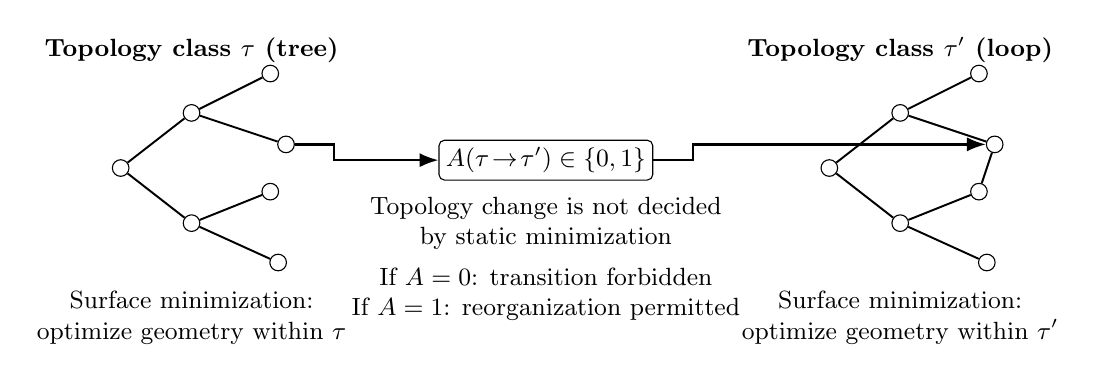
\begin{tikzpicture}[
  x=1cm,y=1cm,
  node/.style={circle,draw,inner sep=1.2pt,minimum size=6pt},
  edge/.style={line width=0.7pt},
  lab/.style={font=\small, align=center}, % Added align=center to allow manual breaks
  title/.style={font=\small\bfseries},
  gate/.style={draw,rounded corners=2pt,inner sep=2.5pt,font=\small},
  arr/.style={-{Latex[length=2.4mm]},line width=0.8pt}
]

% -------------------------
% Panel A: tree-like class
% -------------------------
\node[title] (A_title) at (-4.5,2.3) {Topology class $\tau$ (tree)};
\node[node] (a0) at (-5.4,0.8) {};
\node[node] (a1) at (-4.5,1.5) {};
\node[node] (a2) at (-4.5,0.1) {};
\node[node] (a3) at (-3.5,2.0) {};
\node[node] (a4) at (-3.3,1.1) {};
\node[node] (a5) at (-3.5,0.5) {};
\node[node] (a6) at (-3.4,-0.4) {};

\draw[edge] (a0) -- (a1);
\draw[edge] (a0) -- (a2);
\draw[edge] (a1) -- (a3);
\draw[edge] (a1) -- (a4);
\draw[edge] (a2) -- (a5);
\draw[edge] (a2) -- (a6);

% Added a line break to prevent horizontal clashing
\node[lab] at (-4.5,-1.1) {Surface minimization:\\optimize geometry within $\tau$};

% -------------------------
% Panel B: looped class
% -------------------------
\node[title] (B_title) at (4.5,2.3) {Topology class $\tau'$ (loop)};
\node[node] (b0) at (3.6,0.8) {};
\node[node] (b1) at (4.5,1.5) {};
\node[node] (b2) at (4.5,0.1) {};
\node[node] (b3) at (5.5,2.0) {};
\node[node] (b4) at (5.7,1.1) {};
\node[node] (b5) at (5.5,0.5) {};
\node[node] (b6) at (5.6,-0.4) {};

\draw[edge] (b0) -- (b1);
\draw[edge] (b0) -- (b2);
\draw[edge] (b1) -- (b3);
\draw[edge] (b1) -- (b4);
\draw[edge] (b2) -- (b5);
\draw[edge] (b2) -- (b6);
\draw[edge] (b4) -- (b5);

% Added a line break here as well
\node[lab] at (4.5,-1.1) {Surface minimization:\\optimize geometry within $\tau'$};

% -------------------------
% Middle: admissibility gate
% -------------------------
\node[gate] (G) at (0,0.9) {$A(\tau\!\to\!\tau')\in\{0,1\}$};
\draw[arr] (a4.east) -- ++(0.5,0) |- (G.west);
\draw[arr] (G.east) -- ++(0.5,0) |- (b4.west);

\node[lab] at (0,0.1)
{Topology change is not decided\\by static minimization};

\node[lab] at (0,-0.8)
{If $A=0$: transition forbidden\\If $A=1$: reorganization permitted};

\end{tikzpicture}
\caption{
Schematic illustration of topology selection versus geometric optimization.
Surface minimization determines the optimal geometry within a fixed continuation class (left: tree-like $\tau$, right: looped $\tau'$).
The permissibility of the topology-changing transition $\tau\!\to\!\tau'$ is governed by an admissibility gate $A(\tau\!\to\!\tau')$, which is not determined by the variational principle itself.
}
\label{fig:topology_admissibility}
\end{figure}
Figure~\ref{fig:topology_admissibility} emphasizes that surface minimization ranks geometries within each topology class, while admissibility governs whether transitions between classes occur at all.

The contrast illustrates that the need for an admissibility criterion is not an external imposition on surface-minimization theory, but an implicit requirement already recognized in its application. Surface minimization determines the geometry of configurations conditional on their existence; it does not determine when new configurations become admissible. Making this boundary explicit clarifies the precise limits of the framework's domain of determinacy without diminishing its explanatory power.

\subsection{Implications}

Surface-minimization models occupy a well-defined and powerful position in the theory of physical networks. They provide a necessary description of locally admissible geometry and successfully explain a wide range of observed branching motifs. At the same time, their reliance on a single classical saddle evaluated under fixed constraints renders them generically and structurally incomplete.

The following section identifies the minimal requirements for an additional admissibility principle capable of resolving these undecidable questions while remaining consistent with the empirical successes of surface-minimization approaches.

\begin{center}
\fbox{\parbox{0.92\linewidth}{
\textbf{Main Result.}
Classical surface minimization determines network geometry within a fixed topology class, but it does not determine which topology classes or transitions are physically permitted; therefore any complete theory of physical network organization requires an independent admissibility principle in addition to geometric optimization.
}}
\end{center}

\section{Admissibility as a Necessary Extension}
\label{sec:admissibility}

Section~\ref{sec:incompleteness} established that classical surface-minimization models determine the geometry of locally admissible configurations, but do not determine admissibility itself. In particular, questions concerning topology selection, transition permissibility, and the resolution of conflicting constraints remain undecidable within a framework based solely on classical extrema of a surface-area functional.\cite{Meng2026SurfaceOptimization} This section shows that introducing admissibility as an explicit conceptual layer does more than rename this gap: it resolves concrete indeterminacies left open by surface minimization and leads to distinct, testable consequences.

The purpose here is not to propose a specific admissibility mechanism. Rather, the aim is to demonstrate that admissibility plays a logically irreducible role in completing surface-minimization theories, and to clarify why this role cannot be subsumed by existing optimization-based extensions.

\subsection{Admissibility distinct from optimization}

Surface minimization is an optimization procedure defined over a configuration space assumed to be admissible. It selects an extremal geometry conditional on the existence of that space. Admissibility addresses a different class of questions: whether a configuration is permitted at all, whether a transition between configurations may occur, and whether qualitative reorganization is required under competing constraints.

Formally, admissibility can be represented as a binary relation over continuation classes. Let $\mathcal{T}$ denote the set of candidate topology/continuation classes, and let $A:\mathcal{T}\times\mathcal{T}\to\{0,1\}$ be an admissibility map with $A(\tau\!\to\!\tau')=1$ if the transition $\tau\to\tau'$ is permitted under the relevant constraints and $A(\tau\!\to\!\tau')=0$ otherwise. Surface minimization then determines the extremal geometry \emph{conditional} on $\tau$ and on the admissible transitions encoded by $A$, but does not itself determine $A$. This formulation makes explicit that admissibility is not a graded preference encoded by a cost functional, but a categorical permission structure that partitions configuration space into accessible and forbidden transitions.

This distinction is not merely terminological. Optimization compares alternatives within a fixed domain, whereas admissibility determines the domain itself and governs transitions between distinct domains. Encoding admissibility as a refinement of the surface functional---through additional penalty terms, topology-switching costs, or ensemble weights---does not eliminate this distinction. Such constructions remain optimization-based and therefore presuppose that the relevant configurations and transitions are already admissible. The logical question of whether a transition is permitted in the first place is not answered by assigning it a finite cost.

\subsection{Resolution of indeterminacies left by surface minimization}

The incompletenesses identified in Section~\ref{sec:incompleteness} arise where surface minimization yields determinate geometries but indeterminate physical outcomes. When multiple topologically distinct continuations satisfy the same local constraints, or when capacity constraints conflict across scales, surface minimization remains mathematically well posed yet underdetermined with respect to physical realization.

Admissibility resolves these indeterminacies by introducing categorical distinctions: continuation may be permitted, qualitative reorganization may be required, or a transition may be forbidden. These distinctions are categorical in the sense that they separate mutually exclusive classes of physical behavior---permitted versus forbidden---rather than more-favorable versus less-favorable configurations within a continuous optimization landscape. The outcome is not a small change in geometry, but a change in which configurations or transitions are accessible at all.

\subsection{Admissible transitions and topology change}

A central function of admissibility concerns transitions between distinct configuration classes, particularly those involving topology change. Such transitions are not encoded in static variational formulations, which evaluate extrema within fixed topology classes. Even non-equilibrium or dissipative extensions of variational principles evaluate trajectories within a prescribed configuration space and therefore presuppose the admissibility of the transitions they describe.

While path-integral or ensemble formulations can, in principle, sum over multiple topological sectors, they still require specification of which sectors are included and with what prior weights or measures. That specification is an admissibility decision not determined by the action alone. In particular, choosing which sectors to include and how to weight them already presupposes a prior notion of what transitions are allowed. Surface minimization therefore governs geometry conditional on admissibility, but cannot supply admissibility itself.

\subsection{Illustrative case: history-dependent vascular anastomosis}

The distinct role of admissibility can be illustrated by a minimal schematic example drawn from vascular organization. Consider an initially tree-like vascular network supplying a tissue region. As tissue demand increases or damage occurs, the formation of a loop (anastomosis) between neighboring branches may reduce total surface area and improve flow redundancy.

A surface-minimization analysis performed over both tree-like and looped topologies would predict the looped configuration whenever its minimal area is lower. However, empirical observations indicate that anastomoses form only under specific conditions, such as sustained shear stress, flow-induced vessel wall remodeling, or activation of developmental signaling cascades, and do not appear simply because a looped configuration would be geometrically favorable.\cite{Bentley2014}

This behavior cannot be captured by surface minimization alone. An admissibility constraint---such as a threshold condition on stress accumulation or signaling activation---governs whether the topology switch is permitted. Below threshold, the looped configuration remains physically inaccessible despite being locally optimal; above threshold, topology reorganization becomes admissible, and surface minimization determines which specific anastomotic geometry is realized. The result is path dependence and hysteresis: networks with identical current constraints may exhibit different topologies depending on formation history.

\subsection{Empirical consequences of admissibility}

Introducing admissibility leads to empirical consequences that differ qualitatively from those predicted by optimization alone. These include thresholded topology changes rather than continuous deformation, history-dependent organization under identical boundary conditions, and the persistence of locally non-optimal configurations due to forbidden transitions. In addition, admissibility-driven transitions can produce abrupt reorganization in response to continuous parameter variation, resembling bifurcation-like behavior that is not attributable to instabilities of a potential surface but to crossing admissibility thresholds.

Such features are observed in biological and physical networks and cannot be explained by surface minimization without additional assumptions. Admissibility therefore does not merely label a theoretical gap; it alters the space of expected behaviors in a way that is empirically discriminable.

\subsection{Relation to existing physical principles}

Different systems may realize admissibility through diverse mechanisms, including dynamical stability constraints, developmental regulation, energetic limitations, or evolutionary pressures. These mechanisms are often studied independently and applied in system-specific ways. Abstracting their shared logical role as admissibility clarifies what these mechanisms accomplish when they constrain transitions rather than geometries.

The admissibility concept articulated here is intentionally abstract. It isolates a common decision function that existing principles implement in heterogeneous ways, without asserting that any single mechanism is universal. Surface minimization alone does not supply this function, regardless of how accurately it captures local geometry.

\subsection{Complementarity with surface minimization}

Surface minimization and admissibility occupy complementary but logically non-symmetric roles. Admissibility determines which configurations and transitions are permitted under the relevant constraints. Surface minimization determines the geometry of configurations conditional on admissibility. When conflicts arise, admissibility takes logical precedence by restricting the configuration space over which optimization is performed. Physically, this means that transitions which would reduce surface area may nonetheless be forbidden by developmental, material, or energetic constraints.

Together, the two principles form a layered description of physical network organization. Surface minimization governs shape selection within admissible regimes, while admissibility governs the accessibility of regimes themselves. Neither principle subsumes the other, and both are required for a complete account.

\section{Conclusion}

Surface-minimization models have proven remarkably successful at capturing local geometric motifs in a wide range of physical and biological networks. When formulated as smooth embedded manifolds minimizing an area functional subject to capacity or thickness constraints, these models explain branching angles, asymmetries, and stability regimes with a level of empirical accuracy that earlier wiring-length or one-dimensional optimization theories could not achieve.\cite{Meng2026SurfaceOptimization}

It is important to identify the limits of what surface minimization can decide in principle at the level of the classical variational formulation. When treated as a classical variational theory, surface minimization selects a single extremal configuration within a prescribed topology class and treats capacity constraints kinematically rather than resolving conflicts between competing continuation classes. As a result, questions of topology selection, permissibility of topology-changing transitions, and resolution of incompatible constraints lie outside the formal decision power of surface minimization alone, even under idealized conditions. This structural limitation is not unique to surface minimization, but is a general property of classical variational principles: optimization determines geometry within a prescribed configuration space, but does not determine the admissibility of the configuration space itself.

To resolve these indeterminacies, an additional decision layer is required. We have argued that this layer is best characterized as \emph{admissibility}: a principle governing which configurations and transitions are permitted under competing constraints. Admissibility is logically distinct from optimization and cannot be reduced to a refinement of the optimization functional. It operates categorically rather than incrementally, governs transitions rather than equilibria, and restricts the configuration space over which surface minimization is meaningfully applied. Introducing admissibility does not replace surface minimization; it completes it by specifying the domain within which optimization has determinate meaning.

This distinction leads to qualitative empirical consequences. In regimes where multiple continuation classes coexist, admissibility alters the space of expected behaviors, leading to testable signatures---including thresholded reorganization under continuous parameter variation, path dependence and hysteresis under reversal, and the persistence of locally non-optimal configurations due to forbidden transitions---that are not predictable from static surface minimization alone. Vascular anastomosis provides a canonical illustration of this contrast between geometric optimality and admissible reorganization, consistent with observations from recent three-dimensional imaging studies of vascular remodeling.\cite{Bentley2014} Experimentally, admissibility-governed behavior can be distinguished from pure optimization by protocols that slowly vary a control parameter (e.g., shear stress, growth demand, or pressure) while tracking topology in time: discontinuous or hysteretic topology changes at reproducible thresholds constitute signatures of admissibility, whereas purely optimization-driven geometry would vary continuously.

The admissibility concept articulated in this work is intentionally abstract, and this abstraction is a deliberate scope choice. Different physical systems may realize admissibility through distinct mechanisms---dynamical, developmental, energetic, stochastic, or evolutionary---and this paper does not attempt to unify or formalize those mechanisms. Its contribution is instead to clarify the common \emph{logical role} such mechanisms already play and to show that this role cannot be eliminated or absorbed into surface minimization without loss of explanatory power or predictive scope. In this sense, admissibility plays a role analogous to selection rules in other areas of physics: it determines which configurations or transitions are allowed to enter consideration, without prescribing their detailed dynamics. The present work concerns logical completeness rather than mechanism design; constructing system-specific admissibility criteria is deferred to future domain models. Accordingly, the novelty of the present work is not the observation that classical variational principles possess such structural limits---a point long recognized across physics---but the identification and formalization of this limit in the context of physical and biological network organization, where it has not previously been made explicit.

Thermal or stochastic fluctuations may, in practice, enable rare transitions between configuration classes. Such fluctuation-driven events do not eliminate the need for admissibility; rather, they provide one possible physical mechanism by which admissibility thresholds are crossed. Admissibility remains the logical criterion distinguishing permitted from forbidden transitions, while fluctuations determine how and how often those thresholds are reached.

We emphasize that this work does not propose admissibility as a new fundamental dynamical law, but rather identifies an unavoidable logical role that existing physical, developmental, or material mechanisms already implement in practice.

Although the discussion has focused primarily on biological networks, the admissibility distinction applies equally to other physical systems modeled by constrained minimal surfaces, including material fracture patterns, fluidic transport networks, and engineered microfluidic architectures, wherever topology-changing transitions arise under competing constraints.

Surface minimization and admissibility therefore occupy complementary positions in the theoretical hierarchy. Surface minimization determines geometry within admissible classes, while admissibility determines which classes and transitions are physically available. Both principles are required for a complete theory of physical network organization, and neither subsumes the other. Future work may operationalize admissibility in specific systems, bridging it with dynamical or stochastic models to predict reorganization thresholds and transition boundaries. Formally, surface minimization determines geometry conditional on admissibility, whereas admissibility itself is not derivable from the variational principle and must be specified independently.


% --- Bibliography ---
\bibliographystyle{unsrt}
\bibliography{refs}

\end{document}
